%----------------------------------------------------------------------------------------
%	PACKAGES AND DOCUMENT CONFIGURATIONS
%----------------------------------------------------------------------------------------
\documentclass[11pt]{article}
\usepackage{amsmath} % Required for some math elements
\usepackage{hyperref} 
\usepackage{xcolor}
\usepackage{lipsum} 
\usepackage{cite}
\usepackage{graphicx} % Required for the inclusion of images
\usepackage{algorithmic}
\usepackage{array}
\usepackage{bookmark}
\usepackage{listings}
\usepackage{amssymb}
\usepackage{enumitem}
\usepackage{pythonhighlight}
\usepackage[T1]{fontenc}
\usepackage{inconsolata}
\usepackage[margin=8mm]{geometry}
\usepackage[caption=false, font=footnotesize]{subfig}
\usepackage{fancyhdr}
\pagestyle{fancy}
\lhead{ENGR222 Assignment 3 Submission}
\rhead{Daniel Eisen : 300447549}
\cfoot{\thepage}
\renewcommand{\headrulewidth}{0.4pt}
\renewcommand{\footrulewidth}{0.4pt}

\usepackage[active,tightpage]{preview}
\renewcommand{\PreviewBorder}{1in}
\newcommand{\Newpage}{\end{preview}\begin{preview}}
  


\newlist{steps}{enumerate}{1}
\setlist[steps, 1]{label = Step \arabic*:}

\hypersetup{ %color attributes of citation, link, etc.
    colorlinks=true,
    linkcolor=blue,
    filecolor=gray,      
    urlcolor=blue,
    citecolor=blue,
}

\newcommand{\matlab}{\textsc{Matlab }} %very important and totally necessary addition
 
\newcommand\Item[1][]{%
  \ifx\relax#1\relax  \item \else \item[#1] \fi
  \abovedisplayskip=0pt\abovedisplayshortskip=0pt~\vspace*{-\baselineskip}}
%----------------------------------------------------------------------------------------
%	DOCUMENT INFORMATION
%----------------------------------------------------------------------------------------

\title{ENGR 222 \\ Assignment 3 Submission}
\author{Daniel Eisen : 300447549}
\date{\today}

\begin{document}
\begin{preview}

  \maketitle
  %----------------------------------------------------------------------------------------
  %	DOCUMENT CONTENT
  %----------------------------------------------------------------------------------------

  \begin{enumerate}
    \item \textbf{Multiple Integrals}
          \begin{enumerate}
            \item $f(x,y,z)=xyz \\ G=\{(x,y,z) : xy \le z \le 1,\; 0 \le x \le y,\; 0 \le y \le 1\}$
                  \begin{align*}
                    \iiint_{G} f(x,y,z) \,dV                                                                  & = \int_{0}^{1}\int_{0}^{y}\int_{xy}^{1} xyz \, dz dx dy                                  \\
                                                                                                              & = \int_{0}^{1}\int_{0}^{y}xy\Big| \frac{z^{2}}{2} \Big|_{z=xy}^{z=1} dx dy               \\
                                                                                                              & = \int_{0}^{1}\int_{0}^{y}xy\left( \frac{1}{2} - \frac{x^{2}y^{2}}{2} \right) dx dy      \\
                                                                                                              & = \int_{0}^{1}\int_{0}^{y} \frac{1}{2}(xy-x^{3}y^{3}) dx dy                              \\
                                                                                                              & = \int_{0}^{1} \frac{1}{2} \Big|\frac{x^{2}y}{2}-\frac{x^{4}y^{3}}{4}\Big|_{x=0}^{x=y}dy \\
                    = \int_{0}^{1} \frac{1}{2} \left(\frac{y^{3}}{2}-\frac{y^{7}}{4}\right) dy                & =  \int_{0}^{1} \frac{y^{3}}{4}-\frac{y^{7}}{8} dy                                       \\
                    = \Big| \frac{y^{4}}{16} - \frac{y^8}{64} \Big|_{y=0}^{y=1} = \frac{1}{16} - \frac{1}{64} & = \frac{3}{64}                                                                           \\
                  \end{align*}
            \item Spherical Coordinates: $f(x,y,z)=x \\ G=\{x,y,z \ge 0,\; x^{2}+y^{2}+z^{2} \le 1\}$ \\
                  To find the spherical region bounds, picture the region as an eight of the unit sphere in the all positive octant.
                  $$f(r,\theta,\phi) = r cos(\theta)sin(\phi)$$
                  $$ G = \{(r,\theta,\phi) : r \in [0,1], \theta \in [0, \pi/2], \phi \in [0, \pi/2]\}$$
                  \begin{align*}
                    \iiint_G f(r,\theta,\phi) \,dV  & = \int_{0}^{1}\int_{0}^{\pi/2}\int_{0}^{\pi/2} r cos(\theta)sin(\phi) \,d\phi d\theta dr                                        \\
                                                    & = \int_{0}^{1} r \,dr \int_{0}^{\pi/2} cos(\theta) \,d\theta \int_{0}^{\pi/2} sin(\phi) \,d\phi                                 \\
                                                    & = \frac{r^2}{2}\Big|_{r=1}^{r=0} \times sin(\theta)\Big|_{\theta=0}^{\theta=\pi/2} \times -cos(\phi)\Big|_{\phi=0}^{\phi=\pi/2} \\
                    = \frac{1}{2} \times 1 \times 1 & = \frac{1}{2}
                  \end{align*}
            \item $f(x,y)=y^{-2}e^{-x}  \\ R=\{(x,y) : x \in [0:\infty], y \in [2,\infty] \}$
                  \begin{align*}
                    \iint_{R} f(x,y) \, dA                                     & = \int_{2}^{\infty} \int_{0}^{\infty} y^{-2}e^{-x} \, dxdy                        \\
                                                                               & = \int_{2}^{\infty} y^{-2} dy \int_{0}^{\infty} e^{-x} \, dx                      \\
                                                                               & = \left[-\frac{1}{y}\right]_{2}^{\infty} \times \left[-e^{-x}\right]_{0}^{\infty} \\
                    = \left(0 - -\frac{1}{2}\right) \times \left(0 - -1\right) & = \frac{1}{2}                                                                     \\
                  \end{align*}
            \item Centroid: $R = \{ (r, \theta) : 0 \le r \le \theta, \theta \in [0, 2\pi] \}$
            \begin{align*}
                  x_c &= \frac{1}{|R|} \iint_R r^2cos(\theta) \,dr d\theta\\
                  y_c &= \frac{1}{|R|} \iint_R r^2sin(\theta) \,dr d\theta\\\\
                  |R| &= \frac{1}{2}\int_{0}^{2\pi} \theta^{2} \,d\theta \\
                  &= \left[ \frac{\theta^3}{3} \right]_{0}^{2\pi} = \frac{4\pi^3}{3} \\\\
                  x_c &= \frac{3}{4\pi^3} \int_{0}^{2\pi} \int_{0}^{\theta} r^{2}cos(\theta) \,dr d\theta \\
                  &= \frac{3}{4\pi^3} \int_{0}^{2\pi} \left[ \frac{r^{3}}{3}cos(\theta) \right]_{0}^{\theta} d\theta \\
                  &= \frac{1}{4\pi^3} \int_{0}^{2\pi} \theta^{3}cos(\theta) d\theta \\
                  \mathrm{from \; given:} &= \frac{12\pi^2}{4\pi^3} = \frac{3}{\pi} \\
                  y_c &= \frac{3}{4\pi^3} \int_{0}^{2\pi} \int_{0}^{\theta} r^{2}sin(\theta) \,dr d\theta \\ &\dots \\
                  &=\frac{1}{4\pi^3} \int_{0}^{2\pi} \theta^{3}sin(\theta) d\theta \\
                  \mathrm{from \; given:} &= \frac{12\pi-8\pi^3}{4\pi^3} = \frac{3}{\pi^2} - 2\\
                  \mathrm{centroid} &= \left(\frac{3}{\pi},\frac{3}{\pi^{2}}-2\right)
            \end{align*}
          \end{enumerate}
    \item \textbf{Vector Fields}
          \begin{enumerate}
            \item Divergence: $\textbf{F}=x^{2}y^{3}z^{4}\textbf{i} - xyz\textbf{j} + (x+y+z)\textbf{k}$
                  \begin{align*}
                    \mathrm{div} \; \textbf{F} & = f_{x} + g_{y} + h_{z} \\
                                               & = 2xy^{3}z^{4} -yz + 1  \\
                  \end{align*}
            \item Curl: $\textbf{F}=x^{2}y^{3}z^{4}\textbf{i} - xyz\textbf{j} + (x+y+z)\textbf{k}$
                  \begin{align*}
                    \mathrm{curl} \; \textbf{F} & = (h_y - g_z)\textbf{i} - (f_z - h_x)\textbf{j} + (g_x - f_y)\textbf{k}                      \\
                                                & = (1 + xy)\textbf{i} - (4x^{2}y^{3}z^{3} - 1)\textbf{j} + (-yz - 3x^{2}y^{2}z^{4})\textbf{k} \\
                  \end{align*}
            \item Gradient field: $\phi(x,y,z)=xz^{2}+sin(y)e^{x}$
                  \begin{align*}
                    \nabla_{\phi} & = \phi_{x}\textbf{i} + \phi_{y}\textbf{j} + \phi_{z}\textbf{k}                                                     \\
                                  & =  \left(z^{2} + sin(y)e^{x}\right) \textbf{i} + \left(cos(y)e^{x}\right) \textbf{j} + \left(2xz\right) \textbf{k} \\
                  \end{align*}
            \item Laplacian: $\phi(x,y,z)=xz^{2}+sin(y)e^{x} \; (\mathrm{i.e} \; \nabla{\cdot}\nabla\phi)$
                  \begin{align*}
                    \nabla_{\phi}^{2} & =  \phi_{xx} + \phi_{yy} + \phi_{zz} \\
                                      & =  sin(y)e^{x} - sin(y)e^{x} + 2x    \\
                                      & = 2x
                  \end{align*}
          \end{enumerate}
    \item \textbf{Line Integrals}
          \begin{enumerate}
            \item Calculate $\int_C f \; ds$
                  $$ f(x,y,z) = \frac{y}{x}e^z $$
                  $$C: (x,y,z) = (2t, \; t^2, \; ln(t)) \;\;\mathrm{for} \;\; t \in [1,4]$$
                  \begin{align*}
                    \int_C \frac{y}{x}e^z \,ds                                           & = \int_{1}^{4} \frac{t^2}{2t}e^{ln(t)} \sqrt{x'(t)^{2} + y'(t)^2 + z'(t)^2} \,dt        \\
                                                                                         & = \int_{1}^{4} \frac{t^3}{2t} \sqrt{(2)^{2} + (2t)^2 + \left(\frac{1}{t}\right)^2} \,dt \\
                                                                                         & = \int_{1}^{4} \frac{t^2}{2} \sqrt{4 + 4t^2 + \frac{1}{t^2}} \,dt                       \\
                    = \int_{1}^{4} \frac{t^2}{2} \sqrt{\frac{4t^4 + 4t^2 + 1}{t^2}} \,dt & = \int_{1}^{4} \frac{t^2}{2} \sqrt{\frac{(2t^2 + 1)^{2}}{t^2}} \,dt                     \\
                    = \int_{1}^{4} \frac{t^2}{2} \frac{2t^2 + 1}{t}                      & = \int_{1}^{4} \frac{2t^3 + t}{2} \,dt                                                  \\ \\
                    = \int_{1}^{4} t^3 + \frac{t}{2} \,dt                                & = \frac{t^4 + t^2}{4} \Big|_{1}^{4}                                                     \\
                                                                                         & = (4^4 + 4^2)/4 - (1^4 + 1^2)/4=67.5
                  \end{align*}
            \item Calculate $\int_C \textbf{F} \cdot \; d \textbf{r}$
                  $$ \textbf{F}(x,y,z) = x \textbf{i} - e^{z}\textbf{j} + y \textbf{k} $$
                  $$C: \textbf{r}(t) = 2t \textbf{i} + t^2 \textbf{j} + ln(t) \textbf{k} \;\;\mathrm{for} \;\; t \in [1,4]$$
                  \begin{align*}
                    \textbf{r}'(t)                          & = 2 \textbf{i} + 2t \textbf{j} + \frac{1}{t} \textbf{k}                                                                                                        \\\\
                    \int_C \textbf{F} \cdot \; d \textbf{r} & = \int_{1}^{4} \left(2t \textbf{i} - e^{ln(t)} \textbf{j} + t^2 \textbf{k}\right) \cdot \left(2 \textbf{i} + 2t \textbf{j} + \frac{1}{t} \textbf{k}\right)\,dt \\
                                                            & = \int_{1}^{4} 2(2t) - t(2t) + \frac{1}{t}(t^2) \,dt  = \int_{1}^{4} 5t - 2t^2 \,dt                                                                            \\
                                                            & = \frac{5t^2}{2} - \frac{2t^3}{3} \Big|_{1}^{4} = (5(4^2)/2 - 2(4^3)/3) - (5(1^2)/2 - 2(1^3)/3)=-4.5                                                           \\
                  \end{align*}
            \item Calculate $\int_C \textbf{F} \cdot \; d \textbf{r}$
                  \begin{align*}
                    \phi                                       & = cos(xsin(ye^{z}))                                                                                                                  \\
                    \textbf{F}                                 & = \nabla_{\phi}                                                                                                                      \\
                    \int_C \nabla_{\phi} \cdot \; d \textbf{r} & =\phi(x_1,y_1,z_1) - \phi(x_0,y_0,z_0)                                                                                               \\\\
                    \textbf{r}(t)                              & = \pi cos(\pi t/2)\textbf{i} + \left( \frac{\pi}{2} + sin(8\pi t)\right)\textbf{j} + t(1-t)\textbf{k} \; \mathrm{for} \; t \in [0,1] \\
                    \textbf{r}(0)                              & = \pi cos(0)\textbf{i} + \left( \frac{\pi}{2} + sin(0)\right)\textbf{j} + 0\textbf{k}                                                \\
                                                               & =                                          \pi\textbf{i} + \frac{\pi}{2} \textbf{j} + 0 \textbf{k}                                   \\
                    \textbf{r}(1)                              & = \pi cos(\pi/2)\textbf{i} + \left( \frac{\pi}{2} + sin(8\pi)\right)\textbf{j} + 0\textbf{k}                                         \\
                                                               & =                                           0\textbf{i} +  \frac{\pi}{2}\textbf{j} +  0\textbf{k}                                    \\\\
                    \int_C \nabla_{\phi} \cdot \; d \textbf{r} & =\phi(0,\pi/2,0) - \phi(\pi,\pi/2,0)                                                                                                 \\
                                                               & = cos(0{\times}sin((\pi/2)e^{0}))  - cos(\pi{\times}sin((\pi/2)e^{0}))                                                               \\
                                                               & = 1 - -1 = 2
                  \end{align*}
            \item 
            \begin{align*}
                  \textbf{F}(x,y) &= -2xe^{-x^2}sin(y)\textbf{i} + (1+e^{-x^2}cos(y))\textbf{j} \\
                  f_y &= -2xe^{-x^2}cos(y) \\
                  g_x &= -2xe^{-x^2}cos(y) \\
                  \therefore \; \mathrm{conservative} \\
                  \phi_x = f \therefore \phi &= \int -2xe^{-x^2}sin(y) dx = e^{-x^2}sin(y)+k(y)\\
                  g &= 1+e^{-x^2}cos(y) \\
                  \phi_y &=  e^{-x^2}cos(y)+k'(y) \\
                  \therefore k'(y) &= 1, k(y) = \int 1 \,dy = y + C \\
                  \phi &= e^{-x^2}sin(y) + y + C \\
 \\            \end{align*}
            For any closed curve C, the $\oint \textbf{F}{\cdot}d \textbf{r} = \iint_R (g_x - f _y) dA$, so as \textbf{F} is conservative, thus the integrand is 0. 
          \end{enumerate}
    \item \textbf{Lab Questions}
          \begin{enumerate}
            \item
                  \begin{enumerate}
                    \item \texttt{(x(10), y(10)) = (-2.8179467555071627, -0.31125999010827476)}
                          \begin{center}
                            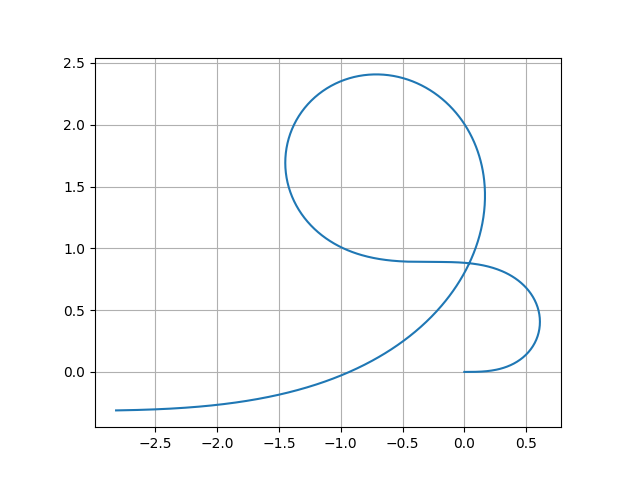
\includegraphics[width=0.33\textwidth]{inc/q4ai.png}
                          \end{center}
                    \item
                          \texttt{h=0.0001: K(s=5) = 1.2001138830544655} \\
                          \texttt{h=0.001: K(s=5) = 1.200113871589581} \\
                          \texttt{h=0.003: K(s=5) = 1.2001137789245757} \\
                          \texttt{h=0.005: K(s=5) = 1.2001135935941987} \\
                          \texttt{h=0.01: K(s=5) = 1.2001127248505328} \\\\
                          $K(s=5) \approx 1.20011$
                  \end{enumerate}
            \item
                  \begin{enumerate}
                    \item \texttt{t = 2: (x,y,z) = (-0.5580567444088435, -0.2720113135900402, 0.11995195426460033)}
                          \begin{center}
                            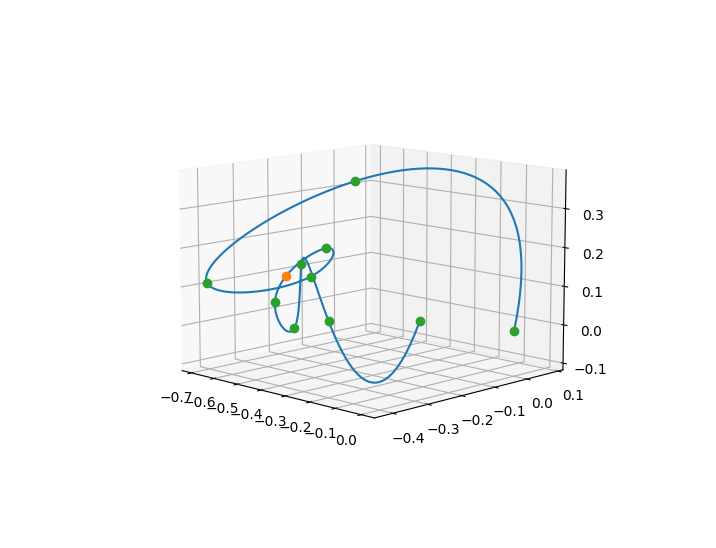
\includegraphics[width=0.5\textwidth]{inc/q4bi_0.png}
                          \end{center}
                    \item unit tangent, principal unit normal and binormal vectors at $t = 2$.
                          \begin{center}
                            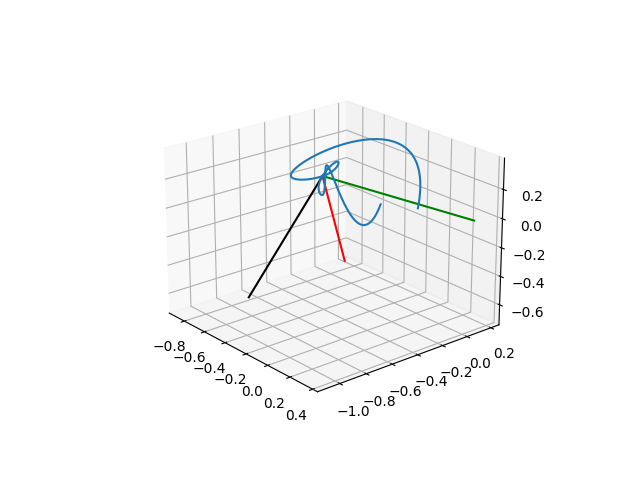
\includegraphics[width=0.5\textwidth]{inc/q4bii.png}
                          \end{center}
                  \end{enumerate}
            \item
                  \begin{enumerate}
                    \item \texttt{result: 8906.117634354589, error: 6.960997495135904e-05}
                    \item \texttt{result: 10.787064853079258, error: 1.1976047768013373e-13}
                  \end{enumerate}
          \end{enumerate}
  \end{enumerate}

  \Newpage

  \inputpython{engr222_ass3_eisendani.py}{1}{1000}

\end{preview}

\end{document}